% \documentclass{article}
%\documentclass[letterpaper, 10 pt, twoside]{IEEEtran}
\documentclass[10pt,twocolumn,letterpaper]{article}
\usepackage[a4paper, total={18cm, 26cm}]{geometry}
\usepackage[utf8]{inputenc}

%\usepackage{float}
\usepackage{graphicx}
\usepackage{amsmath}
\usepackage{amssymb}
\usepackage{booktabs}
\usepackage{nicefrac}
\usepackage{algorithm}
\usepackage[algo2e]{algorithm2e} 
\usepackage{multirow}
\usepackage[pagebackref,breaklinks,colorlinks]{hyperref}
\usepackage{float}

% Support for easy cross-referencing
\usepackage{graphicx}
\usepackage{amsmath}
\usepackage{multirow}
\usepackage[capitalize]{cleveref}
\crefname{section}{Sec.}{Secs.}
\Crefname{section}{Section}{Sections}
\Crefname{table}{Table}{Tables}
\crefname{table}{Tab.}{Tabs.}

\title{Initiation à la recherche : Examen final}
\author{Alexandre Riffard
}
% \date{.....}
% \nocite{*}

\begin{document}

\maketitle
% \abstract{
% Your abstract here
% }
\nocite{*}


\begin{figure*}
    \centering
    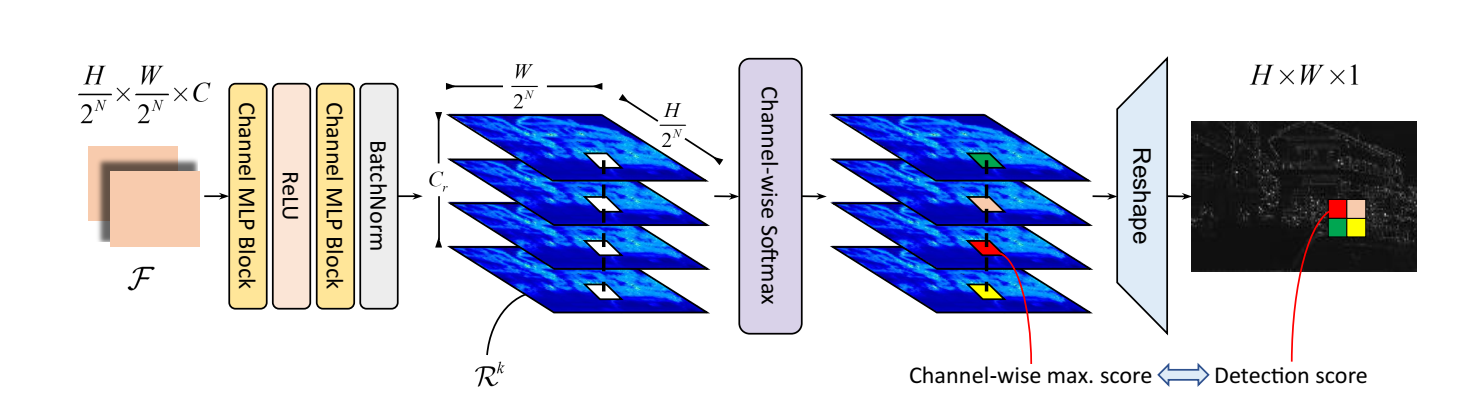
\includegraphics[width=17cm]{images/fig3.png}
    %\captionsetup
    \caption{\textbf{Detection module.} The learned feature representations of the input image is processed by two channel-wise MLP blocks. The keypoints are then detected by using channel-wise softmax operation and mapped back to the original image domain.}
    \label{fig:Fig3}
\end{figure*}

\noindent ing Gaussian kernels at those locations. The loss function used to train the network can be formalized described as:
\begin{equation}
        \mathcal{L} = ||\mathcal{R} + \mathcal{R}_{GT}||^2,
\end{equation}
where $\mathcal{R}$ is the predicted response map (as shown in \cref{fig:2a}) and $\mathcal{R}_{GT}$ is the ground truth response map.
\section{Experiments}
The main motivation of our work is to develop a motion blur aware local feature detector via deep networks, since many state-of-the-art methods for a sharp image have been proposed and achieved impressive performance. There is no existing dataset to evaluate local feature detectors on motion blurred images. We thus create a training dataset via a publicly available single image deblurring dataset, \textit{i.e.} the GoPro dataset from Nah \textit{et al.} [40] which has paired sharp and
blurred images. To evaluate our method, we generate a synthetic dataset via HPatches dataset [5] , which is commonly used for local feature evaluations. HPatches dataset is different from the GoPro dataset, and it can thus also reflect the generalization performance of our method. We therefore mainly use this dataset for evaluation.

\paragraph{Dataset.}
We use the GoPro dataset from Nah \textit{et al.} [40] to generate data to train our network. The GoPro dataset is commonly used for evaluations of single image deblurring networks. It consists of 3,214 paired sharp and blurred images, which are captured from 33 scenes. We follow their convention and use 22 sequences for training and 11 sequences for testing. To generate supervision data for each blurred image, we assume the blurred image should have the same keypoint locations as those for its paired sharp image. We use SIFT [34] to first detect keypoints from the sharp image, and then generate a heatmap and place Gaussian kernels as the ground truth response map for network training.

To better evaluate the generalization performance of our method, we generate a synthetic motion blurred image dataset by using HPatches dataset [5]. HPatches dataset is commonly used for local feature evaluations, which orig-
\begin{figure}[H]
    \centering
    \begin{tabular}{cccc}
         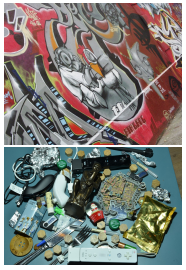
\includegraphics[width=1.75cm]{images/fig_tab1.png} & 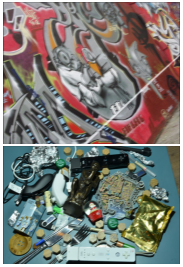
\includegraphics[width=1.75cm]{images/fig_tab2.png} & 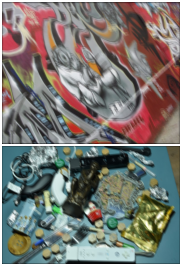
\includegraphics[width=1.75cm]{images/fig_tab3.png} & 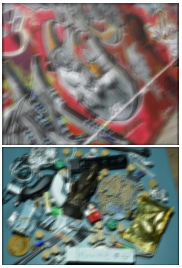
\includegraphics[width=1.75cm]{images/fig_tab4.png}\\
         Sharp & Easy & Hard & Though \\
    \end{tabular}
    \caption{\textbf{Example synthesized blurred images from HPatches dataset [5].} The first column shows the sharp image, and the next three columns are blurred images with varying blur levels. Best viewed in high resolution.}
    \label{fig:Fig4}
\end{figure}
\noindent inally covers both illumination and viewpoint changes. It gathers images from existing datasets, such as DTU [1] and Oxford [39] datasets. It provides a total of 116 sequences and is further divided into 59 sequences for viewpoint changes and 57 sequences for illumination changes. Each sequence includes a reference image and 5 target images with varying viewpoint or illumination changes, together with the corresponding homographies between them. We generate a random motion blur kernel, i.e. point spread function, for each image from the HPatches dataset to synthesize a motion blurred image. We generate three varying levels of motion blur, by changing the blur kernel size and motion irregularities (i.e. the non-linearity of the motion). \cref{fig:Fig4} presents several example images for different blur levels. We use this dataset purely for evaluation.

\paragraph{Implementation details.}
Our network is light-weight
and end-to-end trainable. It requires neither large-scale pretraining nor progressive training. During training, we use a batch size of 4, and Adam optimizer with a initial learning rate of $10^{-4}$. After the network is trained for 20 epochs, we linearly decay the learning rate to $10^{-6}$ till the $50^{th}$ epoch. The network takes about 3 hours to be trained on a single NVIDIA Geforce 2080Ti graphic card. During training, we also perform data augmentation as that of [25].
In particular, we perform a sequence of random rotation, random scaling, random skewing and random perspective transformation on the original image. We also apply random photometric transformation, such that the trained network is robust against illumination changes. Then we randomly crop a 256 × 256 pixels image for training. Detailed network architecture can be found from our supplementary material.

\paragraph{Baseline methods and evaluation metrics.}
We compare our approach against a number of representative detectors, which range from classical handcrafted methods to recent learning based methods. In particular, we compare against SIFT [34], SURF [6], Harris Laplace [38], Shi-Tomasi [56],
MSER [36], KAZE [2], AKAZE [3] and FAST [47] with
their OpenCV implementations. We also compare with
learned feature detectors, such as LIFT [74], Key.Net [25],
SuperPoint [12], LF-Net [41], D2-Net [14], and R2D2 [44].
For fair comparisons with motion blurred images, we also
re-train those learning based methods on the GoPro dataset
using their publicly available source codes. For evaluations
with sharp images, we still use their official provided pretrained models.

The repeatability metric proposed in [37] measures the
quality of keypoint detection and is commonly used by the
community. For a pair of images, it is computed as the ratio
between the number of corresponding keypoints observed
by both images and the smaller number of keypoints detected in one of the two images. To identify the corresponding keypoints, we compute the overlap error, $\epsilon_{I_{o}U}$ is smaller than 0.4, \textit{i.e.} , the overlap between corresponding region is more than $60\%$.

\paragraph{Ablation study}
In this section, we study the effect of the
residual MLP attention block (RMAB). We conduct experiments with three settings, i.e. the network with and without RMAB, and we also replace RMAB with a residual convolutional attention block (RCAB) from [66]. The experimental results shown in \cref{tab:tab1} demonstrate that RMAB block
is indeed effective for local feature detection. The RCAB
block requires more parameters, longer inference time and
achieves lower repeatability compared to the network with
RMAB. It further demonstrates the potential to use MLP
blocks for efficient network architectures. The experiments
are conducted with the GoPro testing sequences.

\paragraph{Evaluation with the original HPatches dataset.}
To study the performance of our method on sharp images, we
compare it against other methods on the original HPatches
dataset [5]. For this experiment, our network is trained on
the GoPro dataset with both sharp and blurred images, while
we use the official pre-trained netwroks for other methods.
Those pre-trained models are usually well trained with a

\begin{table}[H]
    \centering
    \begin{tabular}{cccc} % en mettant "l" au lieu de "c", on a tout aligné à gauche, je suppose que "r" devrait tout aligner à droite
         \hline
         Variant & Repeatability$\uparrow$ & Params$\downarrow$ & Inference time$\downarrow$\\
         \hline
         w/o RMAB & 63.59\% & 326K & 19.18ms \\
         RCAB & 73.56\% & 725K & 57.29ms\\
         RMAB (proposed) & 75.15\% & 381K & 29.02ms\\
         \hline
    \end{tabular}
    \caption{\textbf{Ablation study of the residual MLP attention block
(RMAB).} The experimental results demonstrate that the RMAB
block is indeed efficient and effective for local feature detection.}
    %\captionsetup
    \label{tab:tab1}
\end{table}
\noindent much larger dataset, such as the COCO dataset [31] or the
ImageNet dataset [49]. The experimental results are presented in Tab. 2. It can be demonstrated that our method
performs on-par with the state-of-the-art method (\textit{i.e.} LFNet [41]) for local feature detection with sharp images. Our
method is only slightly worse (\textit{i.e.}$~0.7\%$ drop with the repeatability metric) compared to LF-Net [41], although our
network is trained with a relatively small dataset which contains both sharp and blurred images. The experimental results further demonstrate that our detector (\textit{i.e.} BALF) has
superior performance even it is designed and trained to be
robust against motion blur.

\paragraph{Evaluation with the Blur-HPatches dataset.}
To evaluate the performance of our network with motion blurred
images, we evaluate it against other methods on the synthesized blurred HPatches dataset. For fair comparisons,
we re-train all learning based methods on the same GoPro
dataset. For compactness, we report the total repeatability instead of the separated results for both viewpoint and
illumination changes as in Tab. 3. Detailed results on the
respective changes can be found in our supplementary material. We also simulate two different application scenarios,
\textit{i.e.} the evaluations with blur-to-sharp and blur-to-blur configurations. The blur-to-sharp configuration can be applied
for visual localization task. For example, we can pre-built
a large-scale 3D map with high-quality sharp images. It
might happen that we would use blurred image to query its
location against the 3D map if we walk around with an AR
device at night. The blur-to-blur configuration can be applied for visual odometry task, from which all the captured
images within a time window are motion blurred.

The experimental results shown in Tab. 3 demonstrate
that prior methods have degraded detection performance
when the images are motion blurred. The performance degrades more as the motion blur becomes severer. However,
our method achieves impressive performance compared to
prior works. The reason might be that prior learning based
methods are usually built based on simple convolutional
layers (\textit{e.g.} SuperPoint [12]) or networks which are not specially designed for image deblurring. Motion blurred images thus challenge those networks on keypoint detection
task. In contrary, our network is built based on the multiaxis gated MLP block, which has been demonstrated to be
effective for low-level image processing, \textit{e.g.} image deblurring [64].

\color{blue}
\section{For the new citation (question 7)}
So the first one is about : "Automatic synthesis of realistic images from text". \cite{reed2016generative}
The second one is about STARGAN for image-to-image translation. \cite{choi2018stargan}
The last one is about STARGAN V2 a new version of STARGAN. \cite{choi2020stargan}
\color{black}

{\small
\bibliographystyle{IEEEtran}
%\bibliographystyle{article}
\bibliography{references}
}

\end{document}

